\documentclass[11pt,a4paper]{article}
\usepackage{geometry}
\geometry{top=2.5cm, bottom=2.5cm, left=2.5cm, right=2.5cm}
\usepackage{graphicx}
\usepackage{setspace}
\usepackage{tikz}
\usetikzlibrary{calc}
\usepackage{eso-pic}
\usepackage{titlesec}
\usepackage{float} 
\titleformat{\section}{\fontsize{18pt}{22pt}\bfseries}{\thesection}{1em}{}
\titleformat{\subsection}{\fontsize{15pt}{19pt}\bfseries}{\thesubsection}{1em}{}

\usepackage{tocloft}
\renewcommand{\cftsecleader}{\cftdotfill{\cftdotsep}}

\usepackage[pagebackref=false]{hyperref}
\hypersetup{
    colorlinks=true,
    linkcolor=blue,
    citecolor=blue,
    urlcolor=blue
}

\usepackage{xepersian}
\settextfont[
    Path = fonts/ ,
    Extension = .TTF
]{XB Niloofar}

\usepackage{booktabs}
\usepackage{listings}
\setlatintextfont{Times New Roman} 
\begin{document}

\AddToShipoutPictureBG{
    \begin{tikzpicture}[remember picture, overlay]
        \node[draw, line width=2.5pt, minimum width=\paperwidth-2cm, minimum height=\paperheight-2cm, inner sep=0pt] at (current page.center) {};
        \node[draw, line width=1.0pt, minimum width=\paperwidth-2.3cm, minimum height=\paperheight-2.3cm, inner sep=0pt] at (current page.center) {};
    \end{tikzpicture}
}

\begin{titlepage}
    \centering
    \vspace*{0.5cm}
    
\includegraphics[width=3.5cm]{images/logo.png} \\[0.6cm]
    {\fontsize{14pt}{18pt}\selectfont دانشگاه صنعتی شریف} \\[0.2cm]
    {\fontsize{14pt}{18pt}\selectfont دانشکده مهندسی کامپیوتر}

    \vspace{2.5cm}
    {\fontsize{12pt}{16pt}\selectfont عنوان:} \\[0.5cm]
    {\fontsize{22pt}{28pt}\bfseries طراحی یک انکوباتور } \\[0.4cm]
    
    \vspace{1.5cm}
    {\fontsize{12pt}{16pt}\selectfont نام درس} \\[0.4cm]
    {\fontsize{14pt}{18pt}\bfseries آزمایشگاه طراحی سامانه های رقمی  }

    \vspace{1.5cm}
    {\fontsize{12pt}{16pt}\selectfont نیم‌سال ۱۴۰۴۳}

    \vspace{1.5cm}
    {\fontsize{12pt}{16pt}\selectfont استاد} \\[0.4cm]
    {\fontsize{14pt}{18pt}\bfseries دکتر اجلالی}

\vspace{1.5cm}
{\fontsize{12pt}{16pt}\selectfont گروه 2\par}
\vspace{0.4cm}
{\fontsize{14pt}{20pt}\bfseries
علی سلطانی - 403106092\\[0.2cm]
یگانه کربلایی - 403106527\\[0.2cm]
محمدمهدی مرادی - 403106681\par}

    \vfill
\end{titlepage}

\newpage
\tableofcontents
\newpage

\section{هدف آزمایش}
هدف این آزمایش، طراحی و پیاده‌سازی واحد کنترل رقمی \LTRfootnote{Digital} یک سامانه انکوباتور\LTRfootnote{Incubator} رقمی  است. این واحد باید بر اساس دمای دریافتی از یک حسگر\LTRfootnote{Sensor} ۸ بیتی علامت‌دار، دو ماشین حالت را مدیریت کند: ماشین حالت اصلی که وضعیت روشن/خاموش بودن واحدهای گرم‌کن\LTRfootnote{Heater} و خنک‌کن\LTRfootnote{Cooler} را تعیین می‌کند، و ماشین حالت دوم که سرعت چرخش پنکه\LTRfootnote{Fan} خنک‌کننده را در سه سطح تنظیم می‌کند. علاوه بر این، طرح باید در برابر داده‌های نامعتبر حسگر (خارج از بازه مجاز) مقاوم باشد و با ورود به یک حالت امن\LTRfootnote{Safe State}، از آسیب به سامانه جلوگیری کند. در نهایت، تأثیر روش کدگذاری حالت \lr{(Binary، Gray و One-Hot)} بر منابع منطقی مصرفی و بیشینه بسامد\LTRfootnote{Frequency} کاری مدار سنتزشده بررسی و مقایسه می‌شود.

\section{شرح سامانه و منطق کنترل}

\subsection{ماشین حالت اصلی}
ماشین حالت اصلی سه حالت دارد:
\begin{itemize}
    \item \textbf{\lr{S1} (آماده/خاموش):} هر دو واحد گرم‌کن و خنک‌کن خاموش‌اند. اگر دما بیش از ۳۵ درجه شود به \lr{S2} و اگر کمتر از ۱۵ درجه شود به \lr{S3} می‌رود.
    \item \textbf{\lr{S2} (خنک‌کن روشن):} با کاهش دما به زیر ۲۵ درجه به \lr{S1} بازمی‌گردد.
    \item \textbf{\lr{S3} (گرم‌کن روشن):} با افزایش دما به بالای ۳۰ درجه به \lr{S1} بازمی‌گردد.
\end{itemize}

\subsection{ماشین حالت سرعت خنک کننده}
این ماشین حالت تنها زمانی فعال است که ماشین حالت اصلی در وضعیت \lr{S2} قرار داشته باشد؛ در غیر این صورت بلافاصله به حالت \lr{OUT} (پنکه خاموش) بازمی‌گردد. چهار حالت آن عبارت‌اند از \lr{OUT}، \lr{F1} (۴ دور بر ثانیه)، \lr{F2} (۶ دور بر ثانیه) و \lr{F3} (۸ دور بر ثانیه)، با آستانه‌های گذار ۳۵، ۴۰ و ۴۵ درجه برای افزایش سرعت و ۲۵، ۳۵ و ۴۰ درجه برای کاهش سرعت.

\subsection{واحد نظارت بر سلامت حسگر و حالت امن}
یک نشانک\LTRfootnote{Signal} ترکیبی به‌طور پیوسته بررسی می‌کند که آیا دمای دریافتی در بازه مجاز $[-10, +60]$ قرار دارد یا خیر. به‌محض نامعتبر شدن دما، بدون توجه به حالت جاری، ماشین حالت اصلی بی‌درنگ به حالت \lr{SAFE} می‌رود؛ در این حالت هر دو واحد گرم‌کن و خنک‌کن خاموش شده و نشانک هشدار \lr{error\_sensor} برابر یک می‌شود. بازگشت به کار عادی (حالت \lr{S1}) تنها زمانی رخ می‌دهد که دما مجدداً در بازه مجاز قرار گیرد.

\section{پیاده‌سازی پیمانه کنترل }

\subsection{مشخصه‌ها و کدگذاری حالت‌ها}
دمای ورودی با کلیدواژه \lr{signed} تعریف شده تا مقایسه‌های علامت‌دار (برای دماهای منفی) به‌درستی انجام شود. حالت‌های هر دو ماشین حالت با \lr{localparam} مشخص شده‌اند تا بتوان به‌سادگی روش کدگذاری را برای مقایسه سنتز تغییر داد.

\begin{latin}
\begin{lstlisting}
input  wire signed [7:0] temp;
parameter signed [7:0] TEMP_MIN = -8'sd10;
parameter signed [7:0] TEMP_MAX =  8'sd60;
wire temp_ok = (temp >= TEMP_MIN) && (temp <= TEMP_MAX);

localparam [1:0] MAIN_S1   = 2'b00,  // Idle
                  MAIN_S2   = 2'b01,  // Cooler ON
                  MAIN_S3   = 2'b10,  // Heater ON
                  MAIN_SAFE = 2'b11;  // Safe State
\end{lstlisting}
\end{latin}

\subsection{منطق ترکیبی حالت بعدی}
پیش از بررسی هر یک از حالت‌های عادی، اعتبار دما بررسی می‌شود؛ این کار باعث می‌شود حالت امن\LTRfootnote{Safe State} بر هر منطق دیگری اولویت مطلق داشته باشد. حالت بعدی ماشین سرعت پنکه\LTRfootnote{Fan} نیز بر اساس \lr{main\_next} (نه \lr{main\_state}) محاسبه می‌شود تا بدون تأخیر اضافه، هم‌زمان با خروج از \lr{S2} خاموش شود.

\begin{latin}
\begin{lstlisting}
always @(*) begin
    main_next = main_state;
    if (!temp_ok) begin
        main_next = MAIN_SAFE;
    end else begin
        case (main_state)
            MAIN_S1: begin
                if (temp > 8'sd35)      main_next = MAIN_S2;
                else if (temp < 8'sd15) main_next = MAIN_S3;
            end
            MAIN_S2: if (temp < 8'sd25) main_next = MAIN_S1;
            MAIN_S3: if (temp > 8'sd30) main_next = MAIN_S1;
            MAIN_SAFE: if (temp_ok) main_next = MAIN_S1;
        endcase
    end
end
\end{lstlisting}
\end{latin}

\subsection{منطق ترتیبی و خروجی}
ثبات های حالت در لبه بالارونده ساعت\LTRfootnote{clock} یا با فعال شدن ریست به‌روز می‌شوند. خروجی‌ها به‌صورت \lr{Moore} مستقیماً از حالت جاری تولید می‌شوند؛ در حالت امن، هر دو عملگر خاموش و نشانک\LTRfootnote{Signal} خطا فعال می‌شود.

\begin{latin}
\begin{lstlisting}
always @(posedge clk or posedge rst) begin
    if (rst) begin
        main_state <= MAIN_S1;
        fan_state  <= FAN_OUT;
    end else begin
        main_state <= main_next;
        fan_state  <= fan_next;
    end
end

always @(*) begin
    heater = 1'b0; cooler = 1'b0;
    fan_speed = 2'b00; error_sensor = 1'b0;
    case (main_state)
        MAIN_S2: begin
            cooler = 1'b1;
            case (fan_state)
                FAN_F1: fan_speed = 2'b01;
                FAN_F2: fan_speed = 2'b10;
                FAN_F3: fan_speed = 2'b11;
            endcase
        end
        MAIN_S3: heater = 1'b1;
        MAIN_SAFE: error_sensor = 1'b1;
    endcase
end
\end{lstlisting}
\end{latin}

\section{میزآزمون هوشمند خودکار}
به‌جای اعمال دستی مقادیر دما، میزآزمون\LTRfootnote{TestBench} یک مدل فیزیکی ساده و خطی از محفظه انکوباتور را در یک متغیر از نوع \lr{real} شبیه‌سازی می‌کند: هرگاه گرم‌کن روشن باشد دما با نرخ ثابتی افزایش، و هرگاه خنک‌کن روشن باشد دما متناسب با سرعت پنکه (کم/متوسط/زیاد) کاهش می‌یابد. این مقدار واقعی سپس به یک عدد صحیح ۸ بیتی علامت‌دار تبدیل و به ورودی مدار اعمال می‌شود؛ به این ترتیب یک حلقه بسته کنترل شبیه‌سازی می‌شود.

\begin{latin}
\begin{lstlisting}
always @(posedge clk or posedge rst) begin
    if (rst) begin
        temperature_real <= T_INIT;
    end else begin
        delta = 0.0;
        if (heater) delta = delta + HEAT_RATE;
        if (cooler) begin
            case (fan_speed)
                2'b01: delta = delta - COOL_LOW;
                2'b10: delta = delta - COOL_MED;
                2'b11: delta = delta - COOL_HIGH;
            endcase
        end
        temperature_real <= temperature_real + delta;
    end
end
\end{lstlisting}
\end{latin}

برای بررسی واکنش سامانه به خطای حسگر، در شرح\LTRfootnote{Scenario} آزمون پس از یک دوره کار عادی، دما به‌طور موقت با دستورهای \lr{force}/\lr{release} به مقدار ۱۰۰ درجه (خارج از بازه مجاز) تغییر داده می‌شود و سپس به ۱۰ درجه (داخل بازه مجاز) بازمی‌گردد تا هم ورود به حالت امن و هم خروج از آن آزموده شود.

\section{نتایج شبیه‌سازی در \lr{ModelSim}}

\begin{figure}[H]
    \centering
    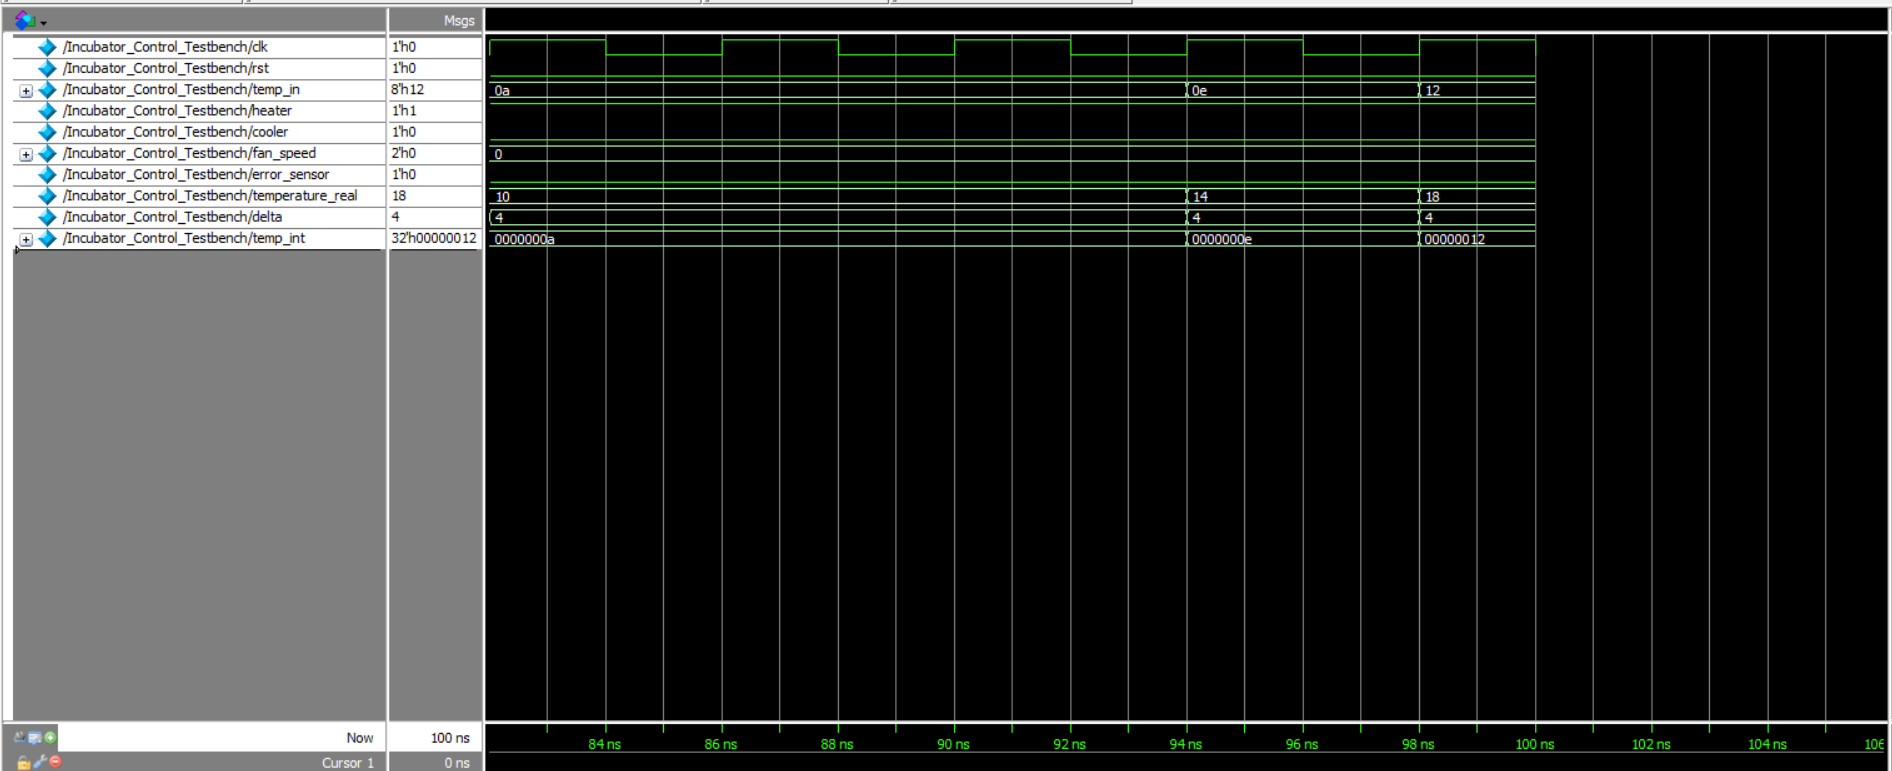
\includegraphics[width=0.95\textwidth]{images/wave_full.png}
    \caption{خروجی کامل شکل موج شبیه‌سازی در \lr{ModelSim}}
    \label{fig:wave-full}
\end{figure}

بخشی از خروجی \lr{Transcript} به‌عنوان نمونه در زیر آمده است (\lr{t} بر حسب نانوثانیه، \lr{T} دمای صحیح اعمال‌شده به مدار):

\begin{latin}
\begin{lstlisting}[numbers=none]
t=2   T=20   Heater=0  Cooler=0  Fan=00  Err=0
t=10  T=20   Heater=0  Cooler=0  Fan=00  Err=0
t=14  T=100  Heater=0  Cooler=0  Fan=00  Err=0
t=18  T=100  Heater=0  Cooler=0  Fan=00  Err=1
...
t=70  T=100  Heater=0  Cooler=0  Fan=00  Err=1
t=74  T=10   Heater=0  Cooler=0  Fan=00  Err=1
t=78  T=10   Heater=0  Cooler=0  Fan=00  Err=0
t=82  T=10   Heater=1  Cooler=0  Fan=00  Err=0
t=94  T=10   Heater=1  Cooler=0  Fan=00  Err=0
t=98  T=14   Heater=1  Cooler=0  Fan=00  Err=0
\end{lstlisting}
\end{latin}

\subsection{تحلیل گام‌به‌گام}
\begin{enumerate}
    \item \textbf{راه‌اندازی ($t=2$ تا $t=10$):} ریست فعال است و مدار در حالت اولیه \lr{S1} با هر دو عملگر خاموش قرار دارد.
    \item \textbf{تزریق خطا ($t=14$):} دمای اعمالی به‌طور ناگهانی به ۱۰۰ درجه (خارج از بازه مجاز $[-10,+60]$) می‌رسد. نشانک \lr{error\_sensor} هنوز صفر است، زیرا محاسبه \lr{main\_next=MAIN\_SAFE} در همین لبه انجام شده اما به ثبات\LTRfootnote{Register} حالت منتقل نشده است؛ این یک دوره\LTRfootnote{Cycle} تأخیر ذاتی، ناشی از منطق ترتیبی همگام با ساعت است.
    \item \textbf{ورود به حالت امن ($t=18$ تا $t=70$):} در لبه بعدی، \lr{main\_state} برابر \lr{MAIN\_SAFE} می‌شود و \lr{error\_sensor=1}. هر دو گرم‌کن و خنک‌کن خاموش باقی می‌مانند؛ این وضعیت تا زمانی که دما نامعتبر است ادامه می‌یابد.
    \item \textbf{بازگشت دما به بازه مجاز ($t=74$):} دما به ۱۰ درجه بازمی‌گردد اما \lr{error\_sensor} همچنان ۱ است، چون \lr{main\_state} هنوز در لبه قبل به‌روز نشده است (همان تأخیر یک دوره ای).
    \item \textbf{خروج از حالت امن ($t=78$):} با به‌روزرسانی ثبات حالت، مدار به \lr{S1} بازمی‌گردد و \lr{error\_sensor=0} می‌شود.
    \item \textbf{ورود به گرمایش ($t=82$):} چون دما (۱۰ درجه) کمتر از ۱۵ است، بلافاصله \lr{main\_next=MAIN\_S3} محاسبه و در لبه بعد اعمال می‌شود؛ \lr{Heater=1} می‌گردد.
    \item \textbf{افزایش دما ($t=98$):} دما از ۱۰ به ۱۴ درجه افزایش می‌یابد. فاصله چند دوره ی بین فعال شدن \lr{Heater} و مشاهده تغییر در \lr{T} ناشی از این است که مدل فیزیکی دما \LTRfootnote{temperature\_real} در یک بلوک \lr{always} جداگانه از ثبات حالت به‌روزرسانی می‌شود و مقدار \lr{heater} یک دوره پیش از اعمال دلتا استفاده می‌شود؛ همچنین تبدیل \lr{real} به عدد صحیح و چاپ \lr{\$display} خود چند مرحله ترکیبی/ثبتی دیگر اضافه می‌کنند. این تأخیرها مربوط به مدل رفتاری محیط شبیه‌سازی است و ارتباطی به صحت منطق کنترلی \lr{FSM} ندارد؛ واکنش خود مدار کنترل (فعال شدن گرم کن) دقیقاً در همان دوره مورد انتظار رخ داده است.
\end{enumerate}


\section{نتایج سنتز و مقایسه روش‌های کدگذاری حالت}
ماشین حالت طراحی‌شده یک‌بار با کدگذاری \lr{Binary}، یک‌بار با \lr{Gray} و یک‌بار با \lr{One-Hot} در نرم‌افزار \lr{Quartus~II} سنتز شد. برای فعال‌سازی تحلیل زمانی، فایل \lr{constraints.sdc} زیر به پروژه افزوده شد:
\begin{latin}
\begin{lstlisting}[numbers=none, language=]
create_clock -name clk -period 20.000 [get_ports clk]
\end{lstlisting}
\end{latin}

\begin{table}[H]
    \centering
    \caption{نتایج سنتز با سه روش کدگذاری حالت}
    \begin{tabular}{lcc}
        \toprule
        روش کدگذاری & تعداد عناصر منطقی \lr{(LE)} & بیشینه بسامد کاری \lr{(MHz)} \\
        \midrule
        \lr{Binary}   & ۴۳ & ۳۱۸.۸۸ \\
        \lr{Gray}     & ۴۳ & ۳۱۸.۸۸ \\
        \lr{One-Hot}  & ۲۹ & ۳۶۴.۳۰ \\
        \bottomrule
    \end{tabular}
    \label{tab:synthesis-results}
\end{table}

\subsection{خروجی‌های روش \lr{Binary}}
\begin{figure}[H]
    \centering
    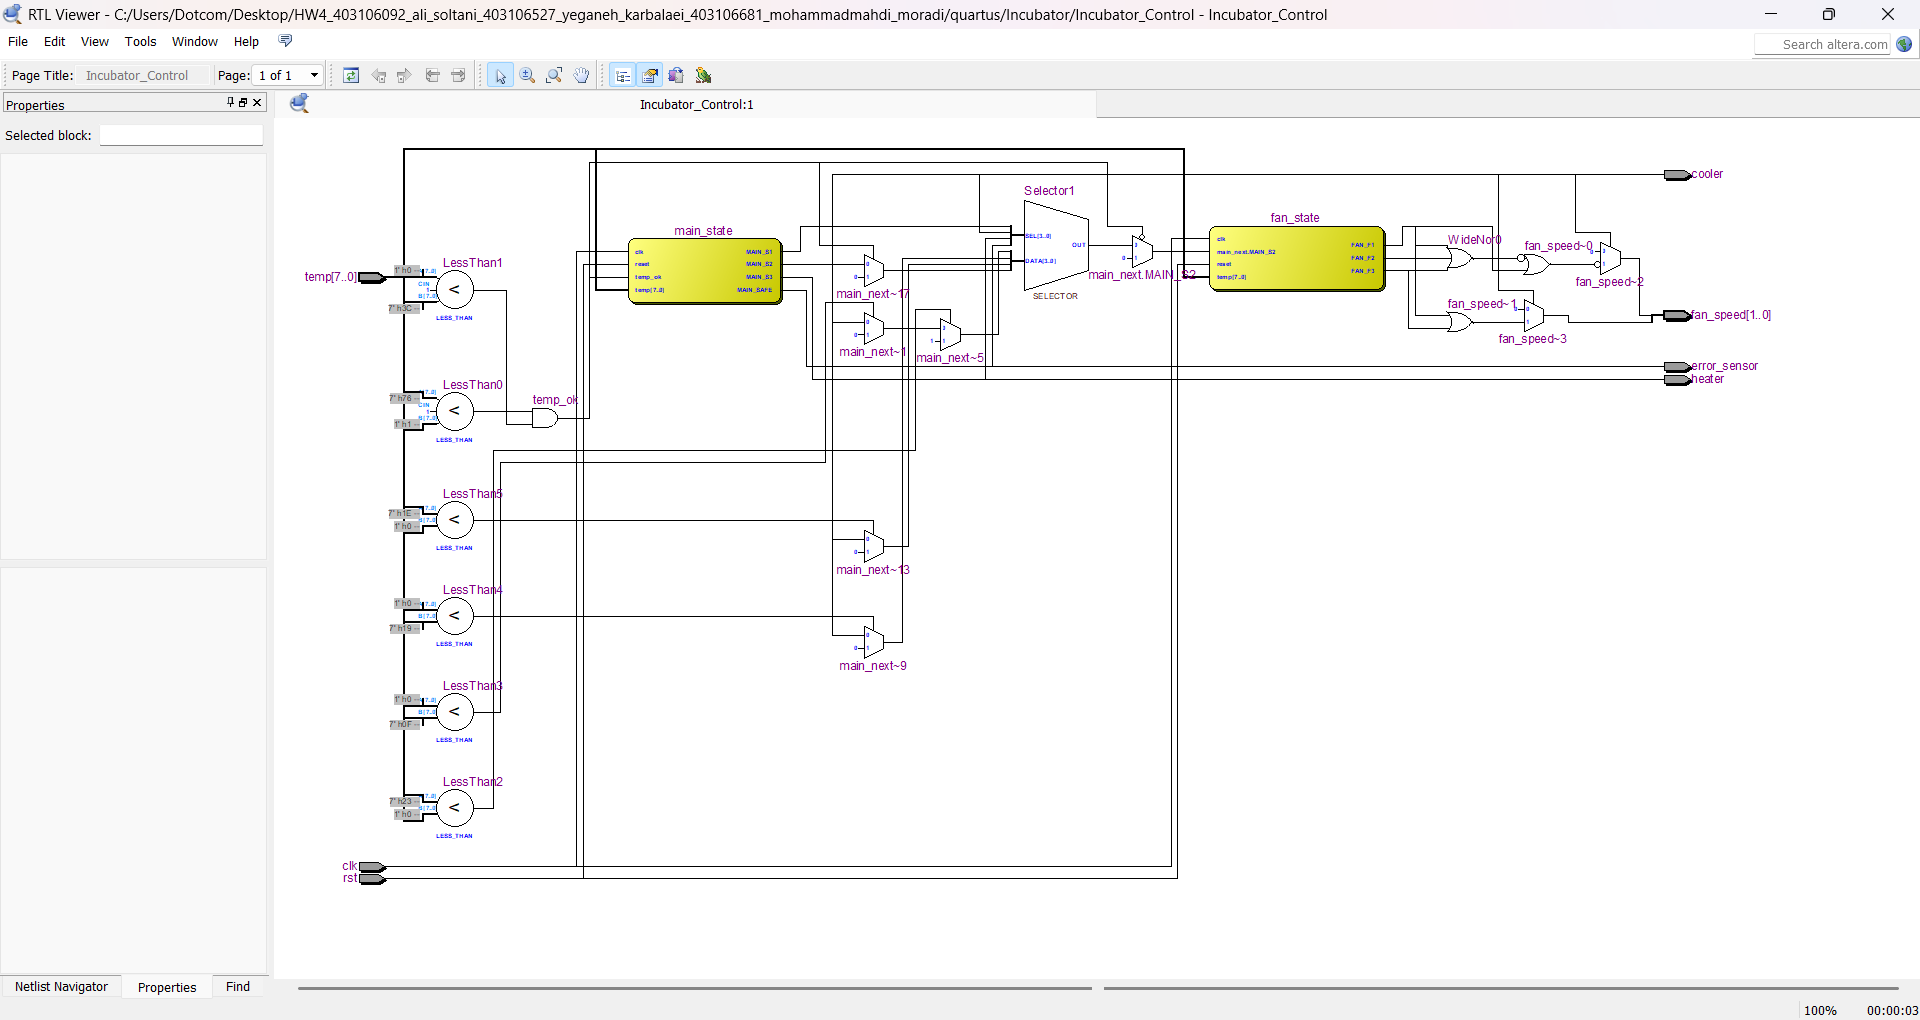
\includegraphics[width=0.9\textwidth]{images/binary/binary_rtl.png}
    \caption{شمای مدار سنتزشده با کدگذاری \lr{Binary}}
\end{figure}
\begin{figure}[H]
    \centering
    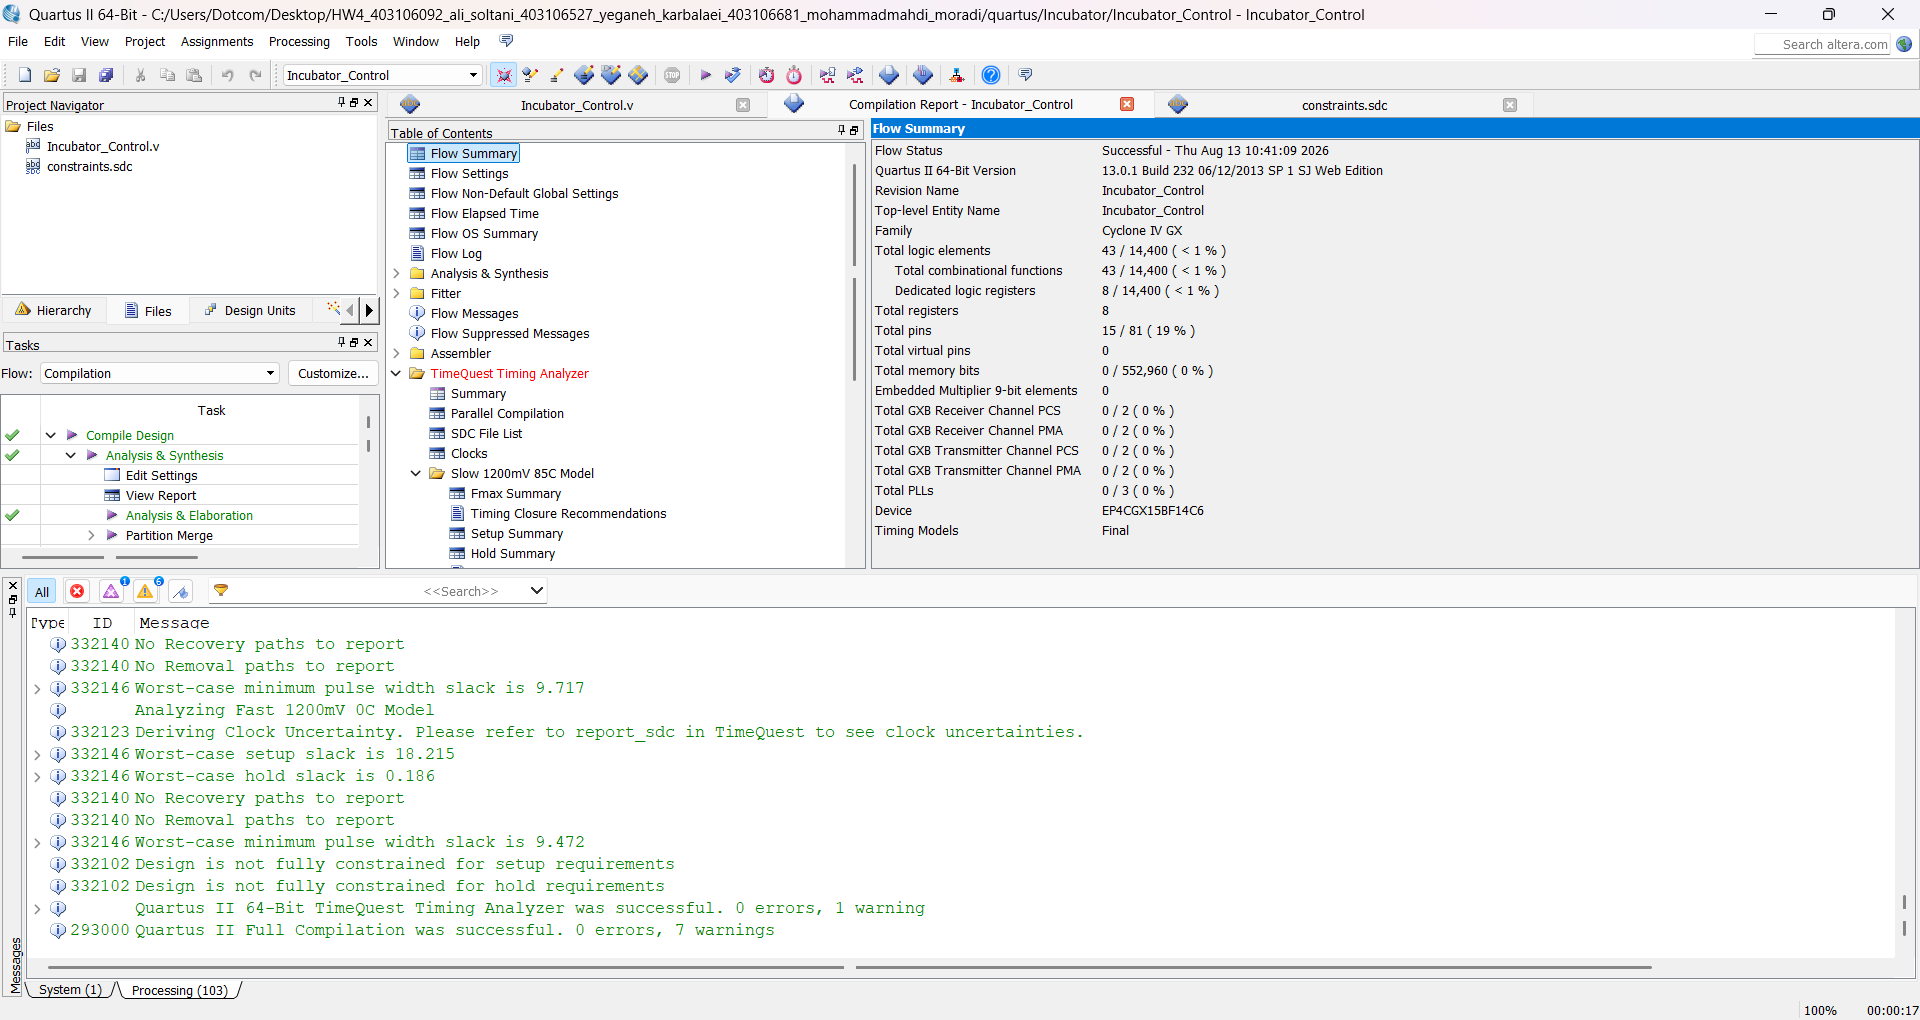
\includegraphics[width=0.9\textwidth]{images/binary/binary_flow_summary.png}
    \caption{تعداد عناصر منطقی مصرف‌شده در کدگذاری \lr{Binary}}
\end{figure}
\begin{figure}[H]
    \centering
    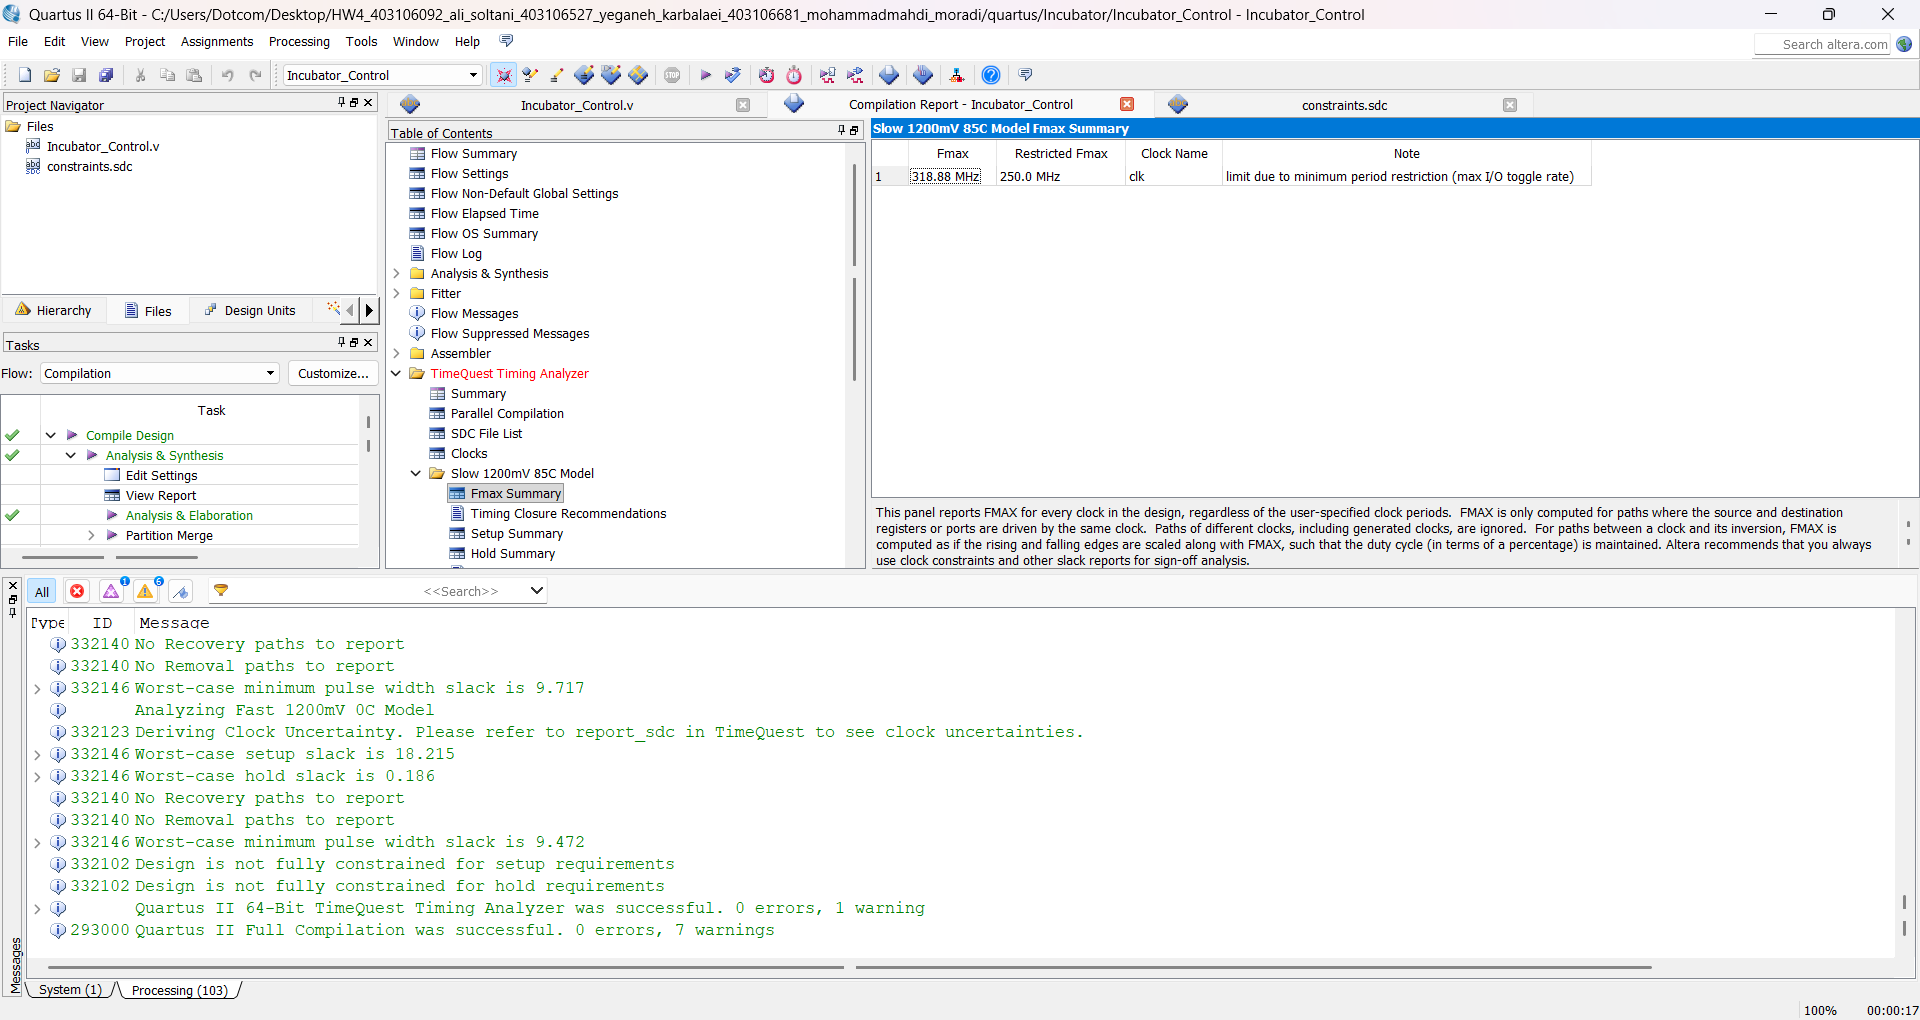
\includegraphics[width=0.9\textwidth]{images/binary/binary_fmax_summary.png}
    \caption{بیشینه بسامد کاری در کدگذاری \lr{Binary}}
\end{figure}
\begin{figure}[H]
    \centering
    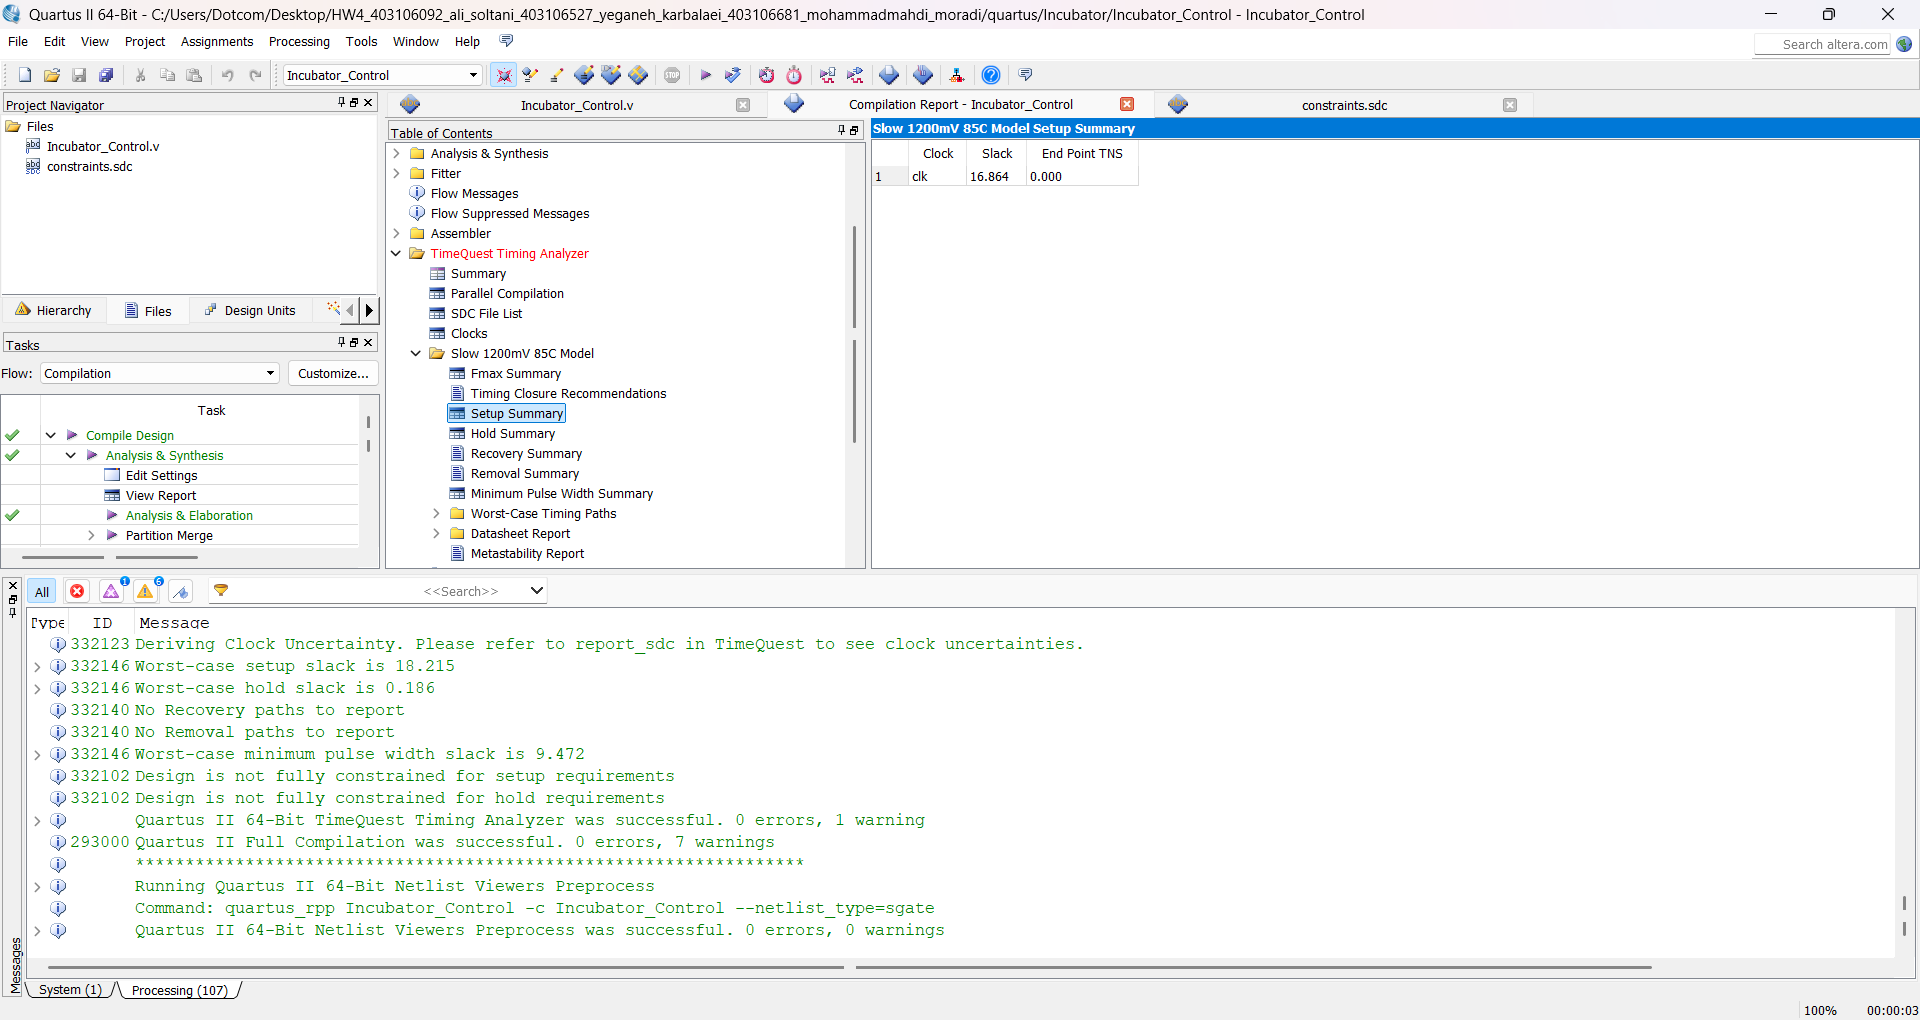
\includegraphics[width=0.9\textwidth]{images/binary/binary_setup_summary.png}
    \caption{بررسی \lr{Worst-case slack} در کدگذاری \lr{Binary} روی ساعت  \lr{50 MHz}}
\end{figure}

\subsection{خروجی‌های روش \lr{Gray}}
\begin{figure}[H]
    \centering
    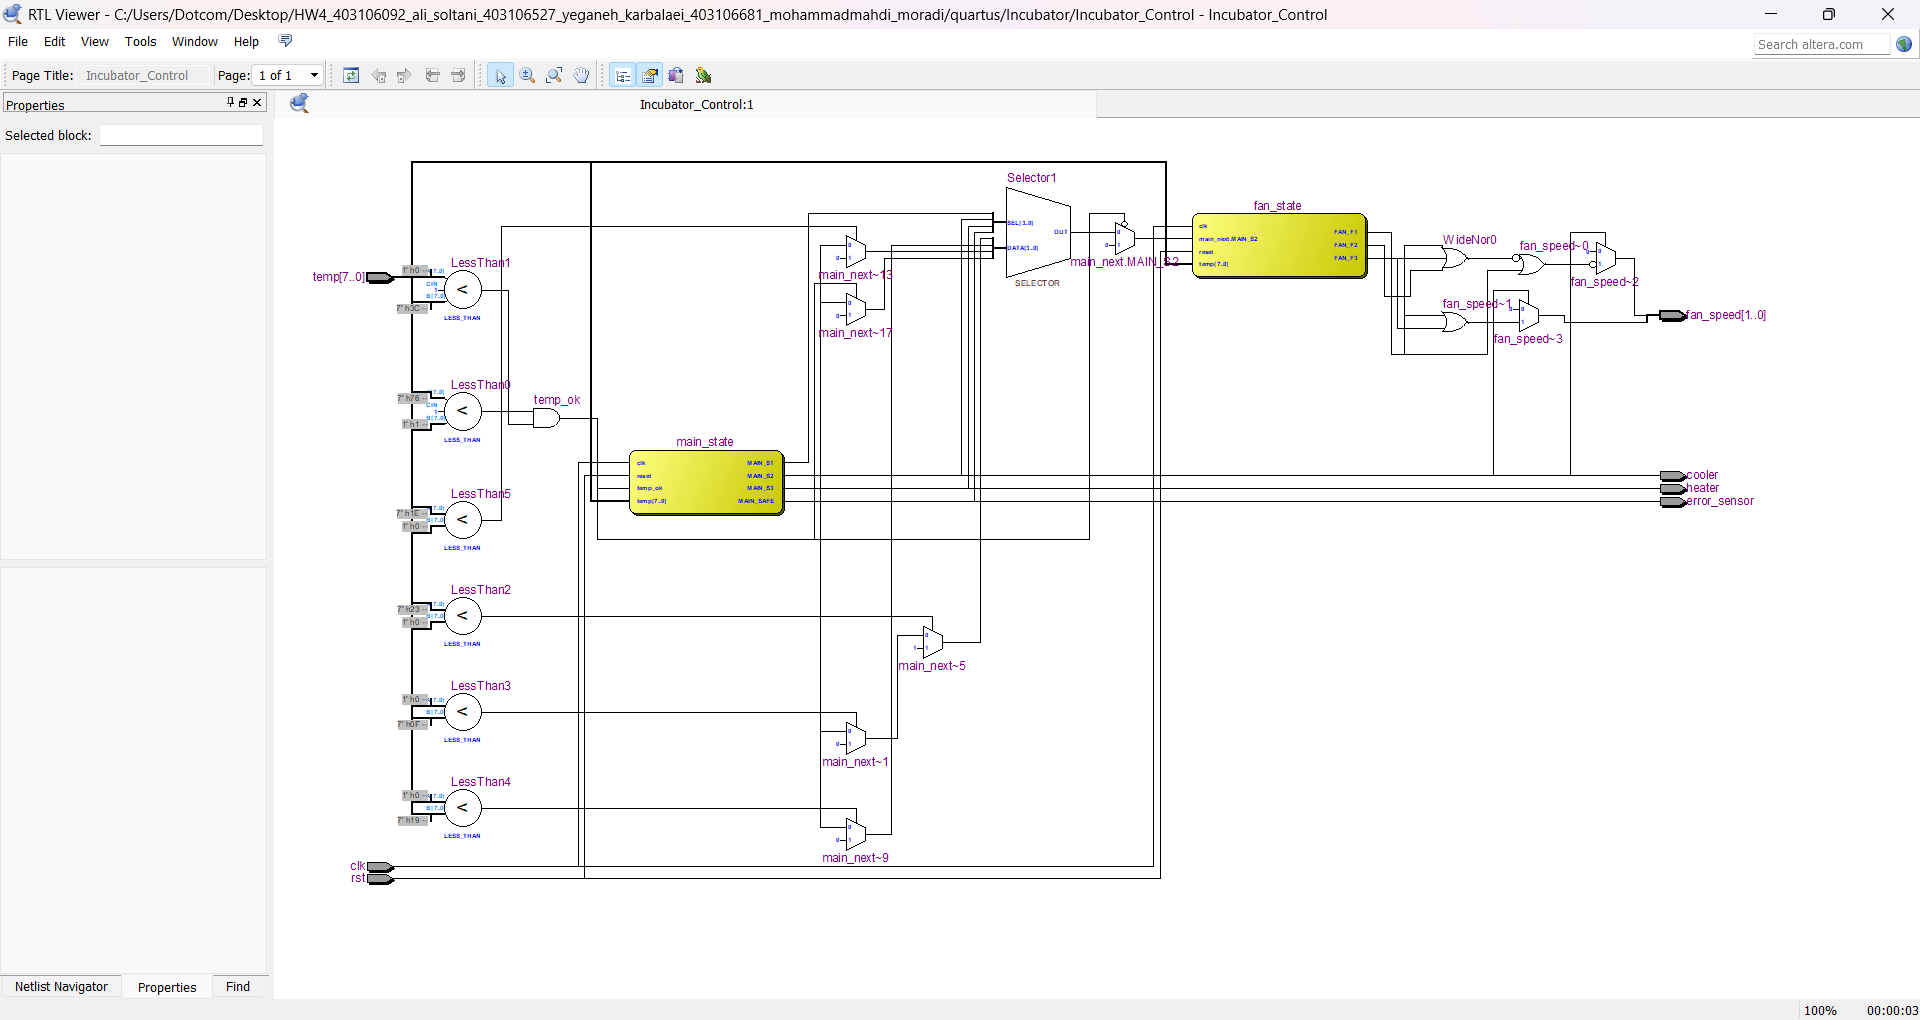
\includegraphics[width=0.9\textwidth]{images/gray/gray_rtl.png}
    \caption{شمای مدار سنتزشده با کدگذاری \lr{Gray}}
\end{figure}
\begin{figure}[H]
    \centering
    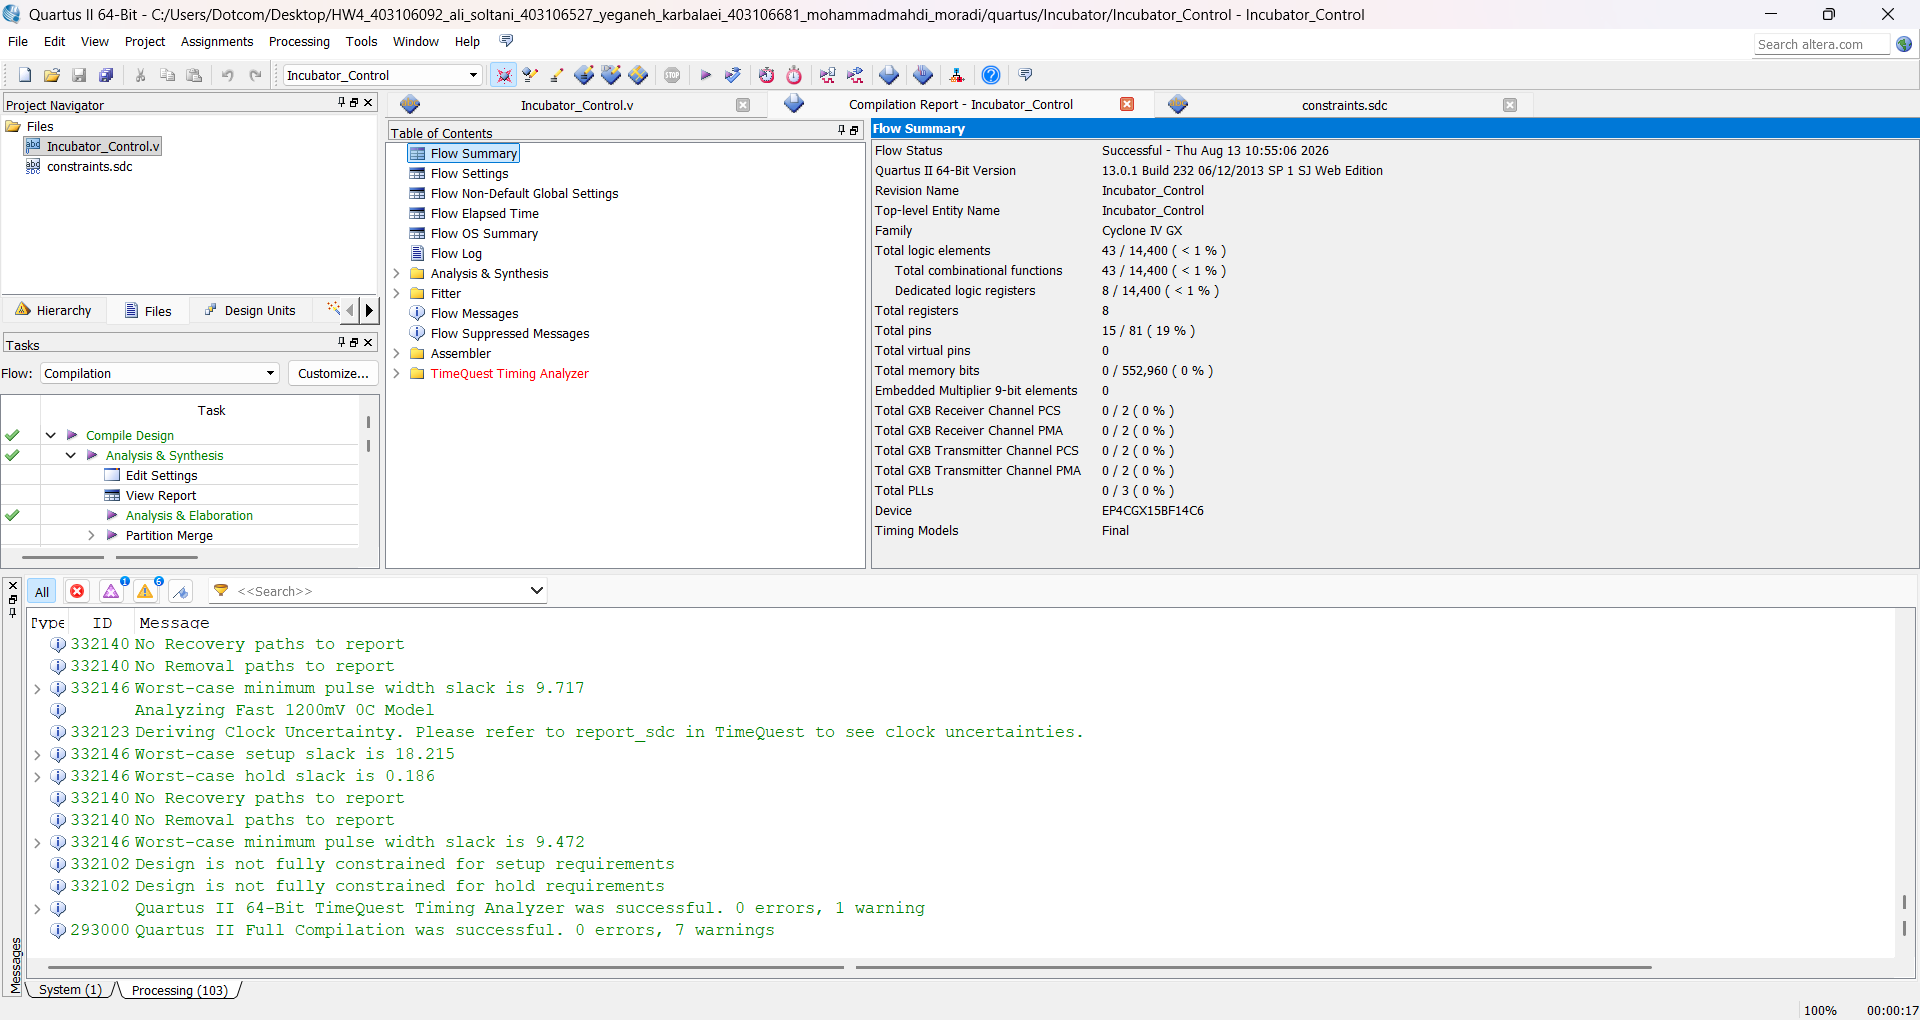
\includegraphics[width=0.9\textwidth]{images/gray/gray_flow_summary.png}
    \caption{تعداد عناصر منطقی مصرف‌شده در کدگذاری \lr{Gray}}
\end{figure}
\begin{figure}[H]
    \centering
    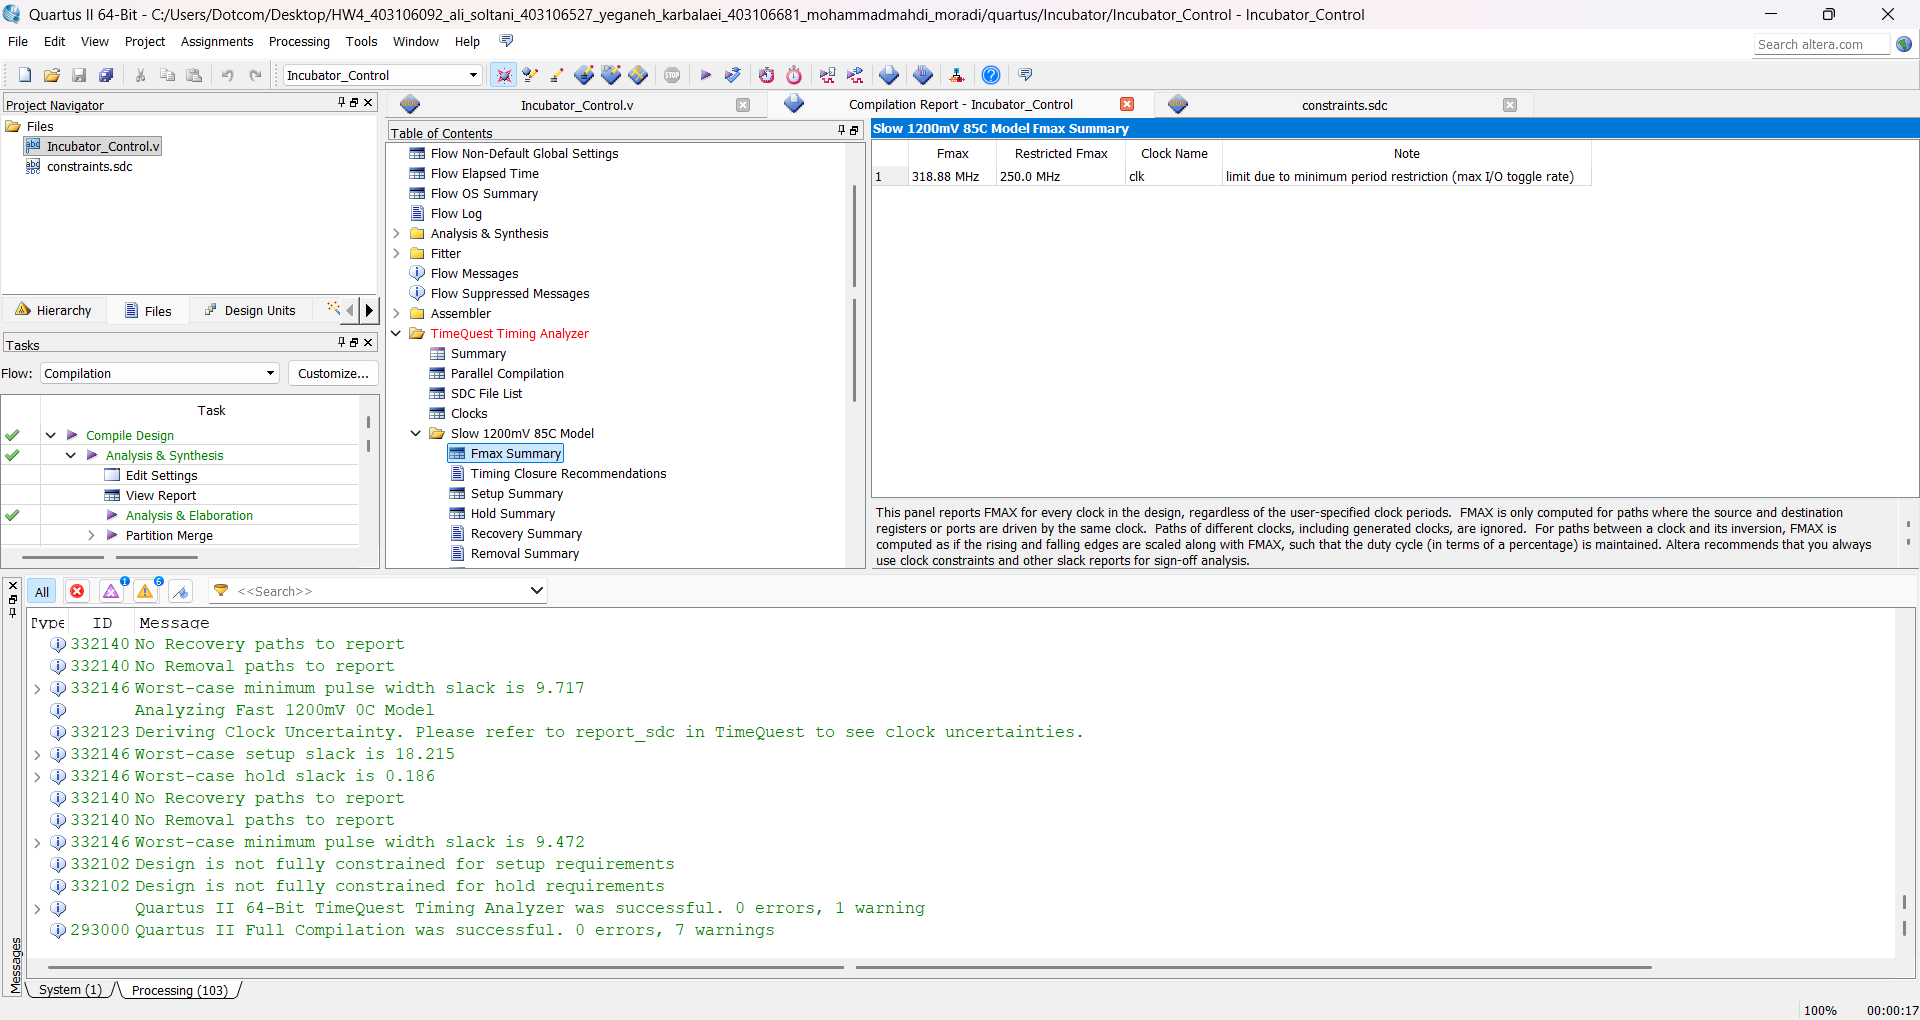
\includegraphics[width=0.9\textwidth]{images/gray/gray_fmax_summary.png}
    \caption{بیشینه بسامد کاری در کدگذاری \lr{Gray}}
\end{figure}
\begin{figure}[H]
    \centering
    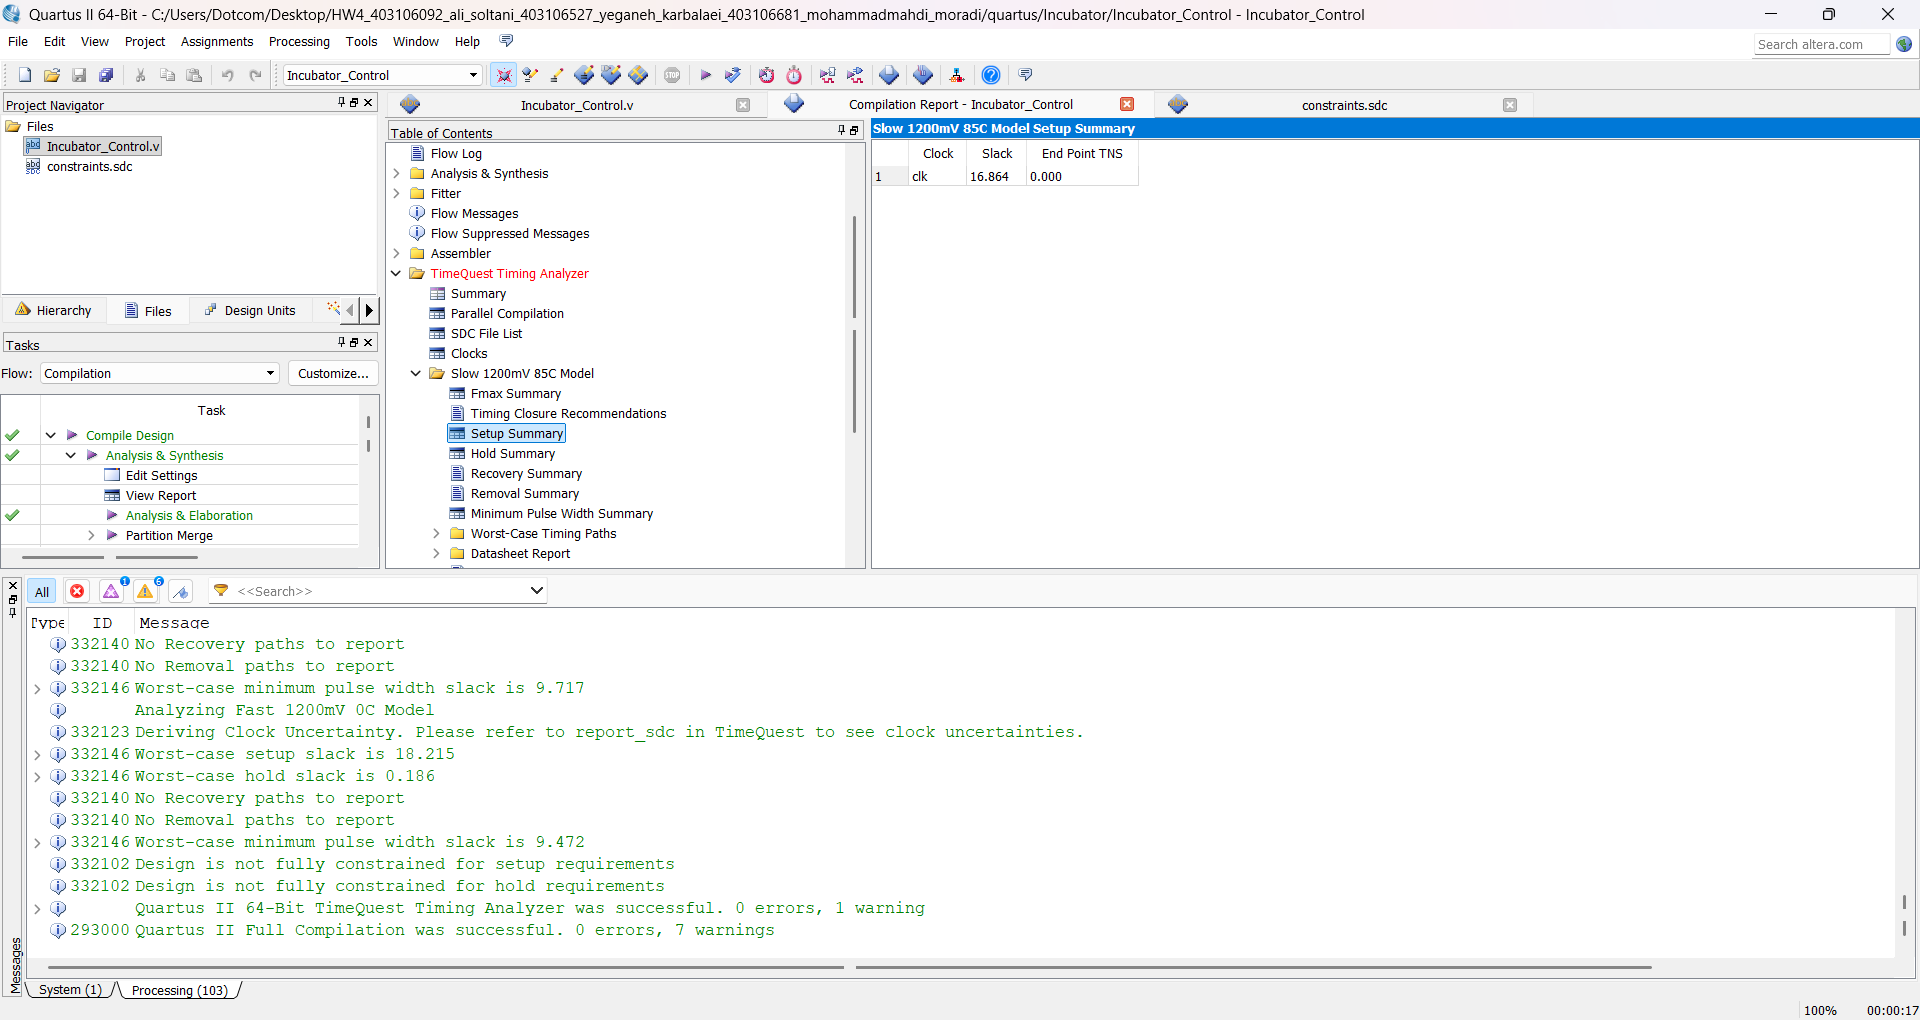
\includegraphics[width=0.9\textwidth]{images/gray/gray_setup_summary.png}
    \caption{بررسی \lr{Worst-case slack} در کدگذاری \lr{Gray} روی ساعت \lr{50 MHz} }
\end{figure}

\subsection{خروجی‌های روش \lr{One-Hot}}
\begin{figure}[H]
    \centering
    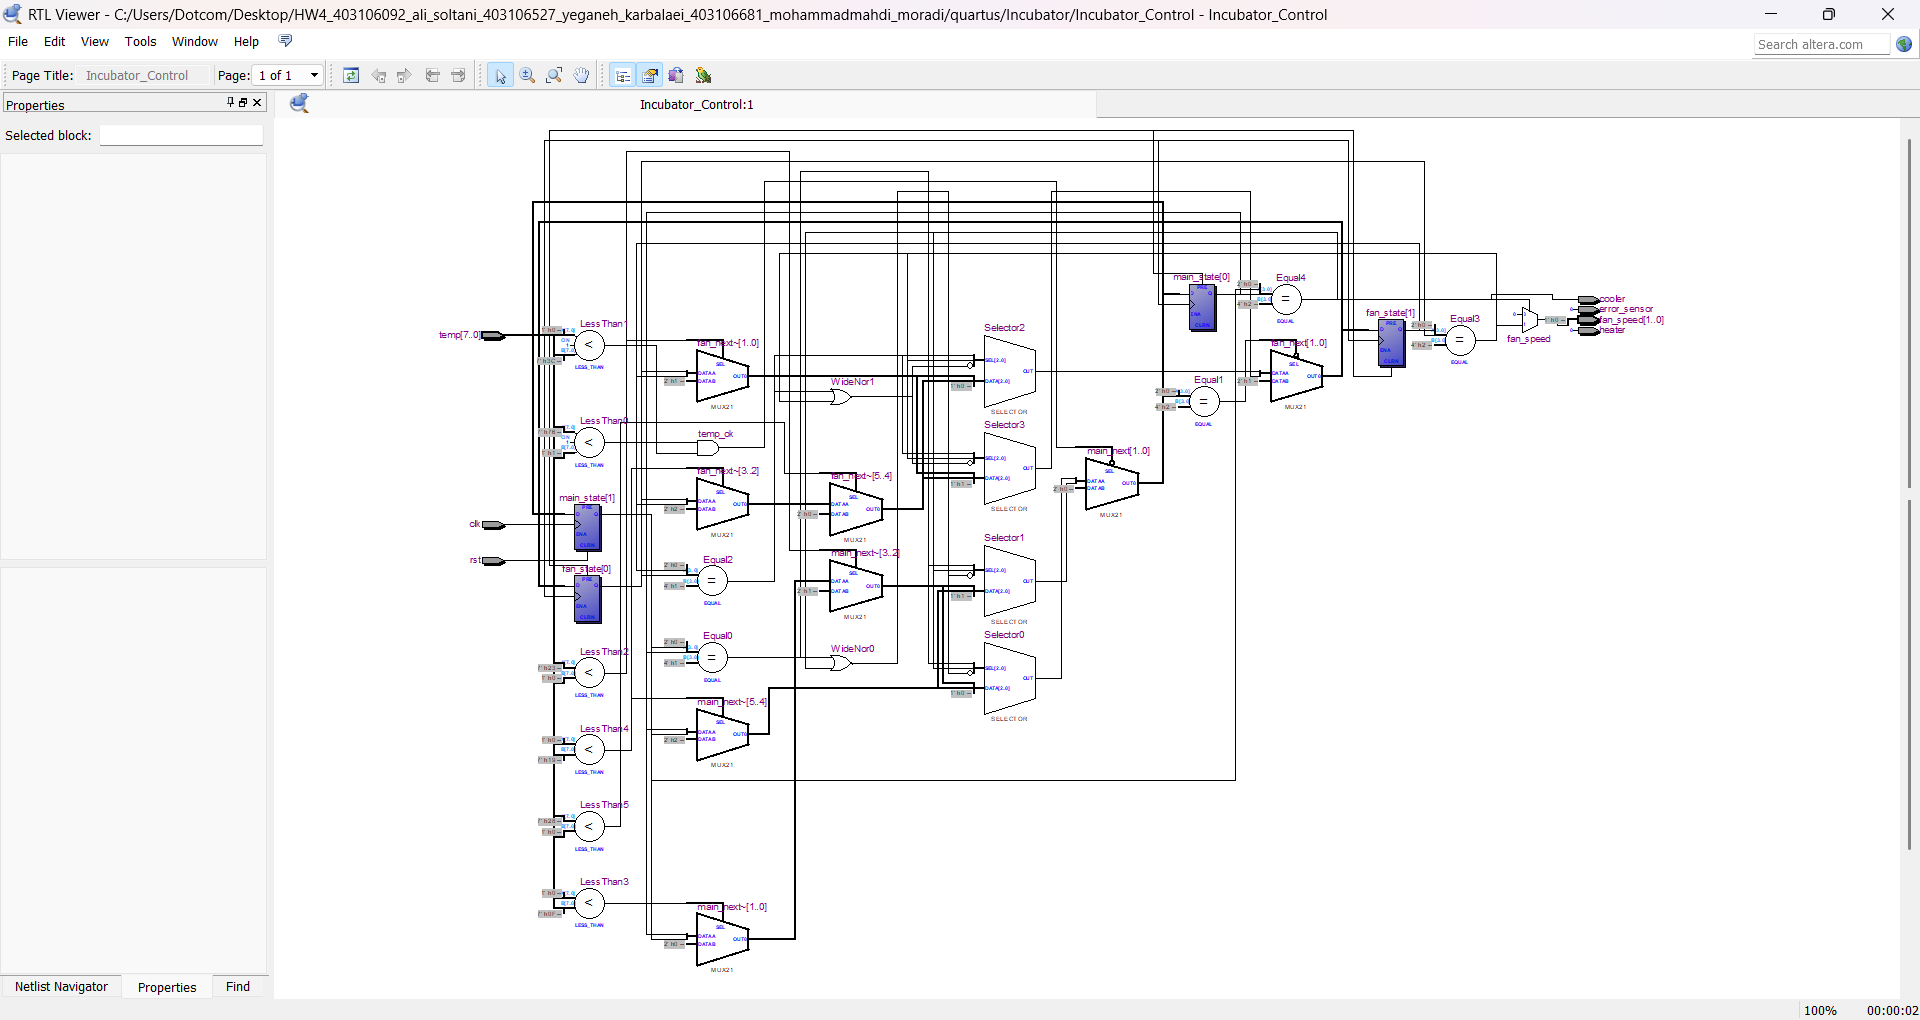
\includegraphics[width=0.9\textwidth]{images/onehot/onehot_rtl.png}
    \caption{شمای مدار سنتزشده با کدگذاری \lr{One-Hot}}
\end{figure}
\begin{figure}[H]
    \centering
    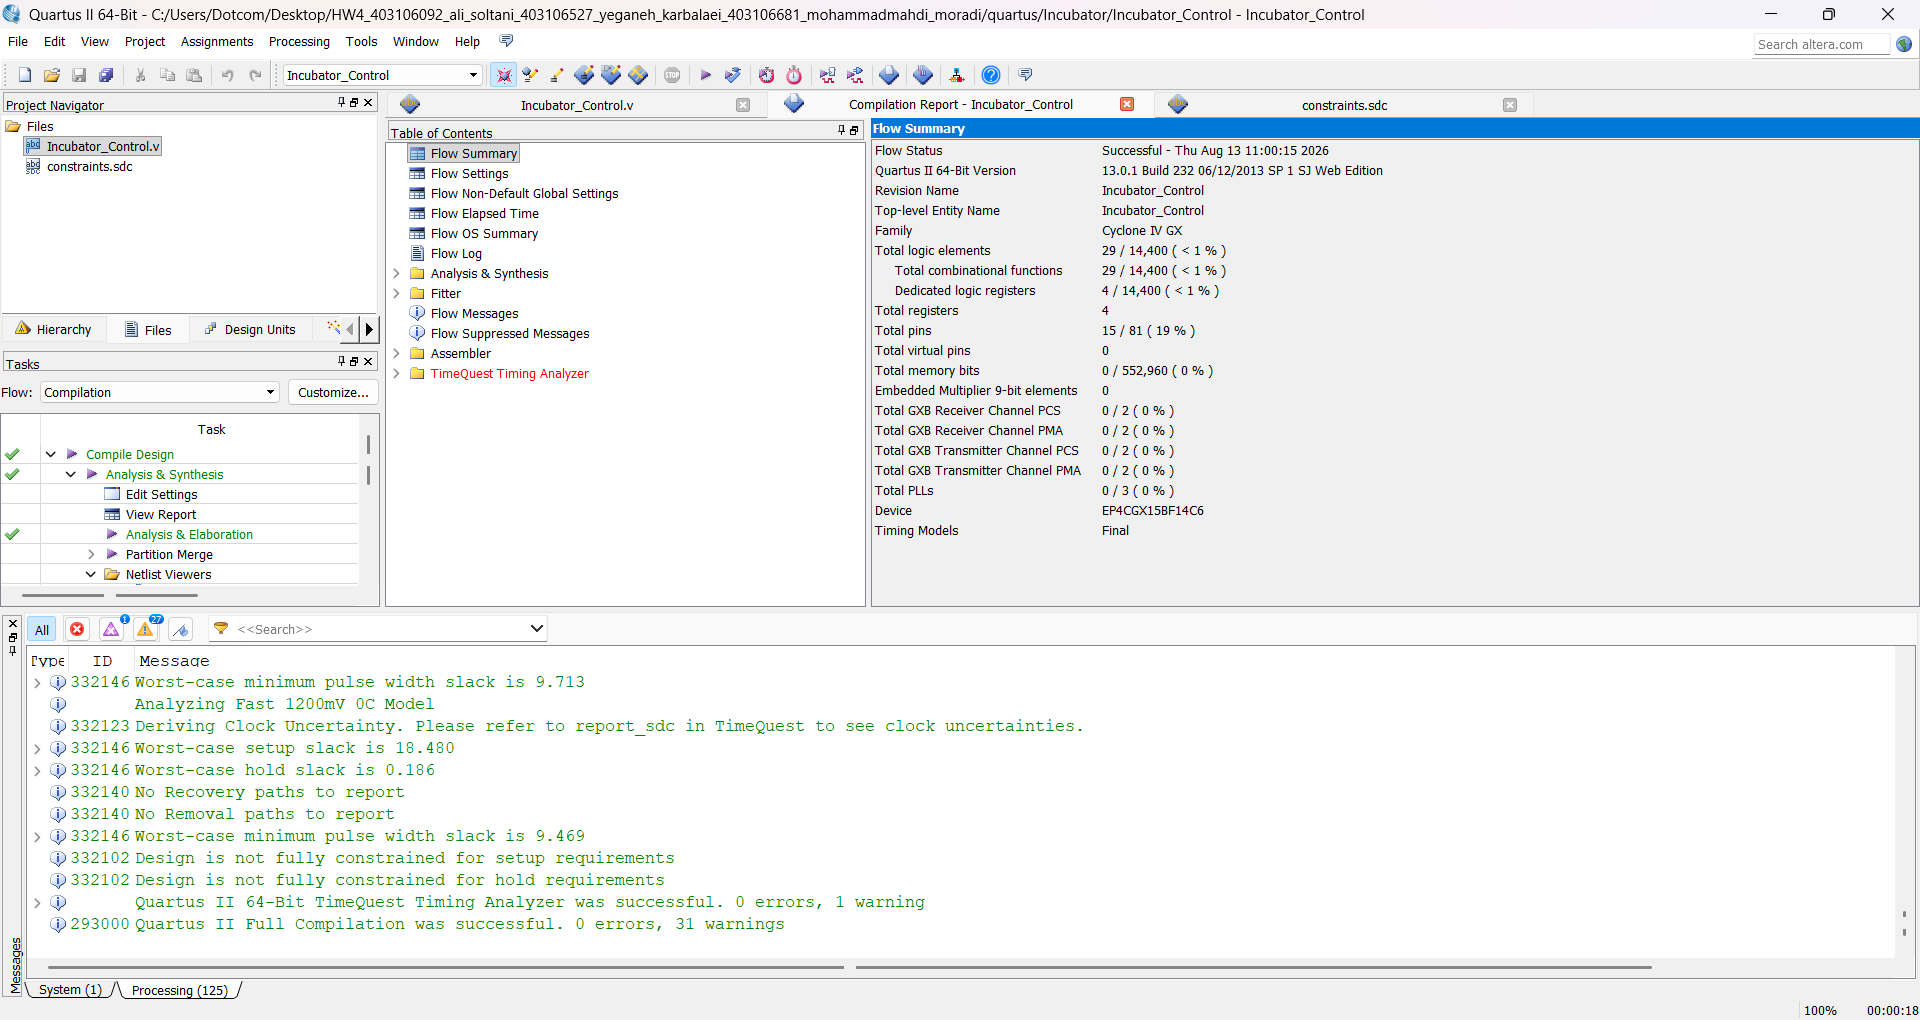
\includegraphics[width=0.9\textwidth]{images/onehot/onehot_flow_summary.png}
    \caption{تعداد عناصر منطقی مصرف‌شده در کدگذاری \lr{One-Hot}}
\end{figure}
\begin{figure}[H]
    \centering
    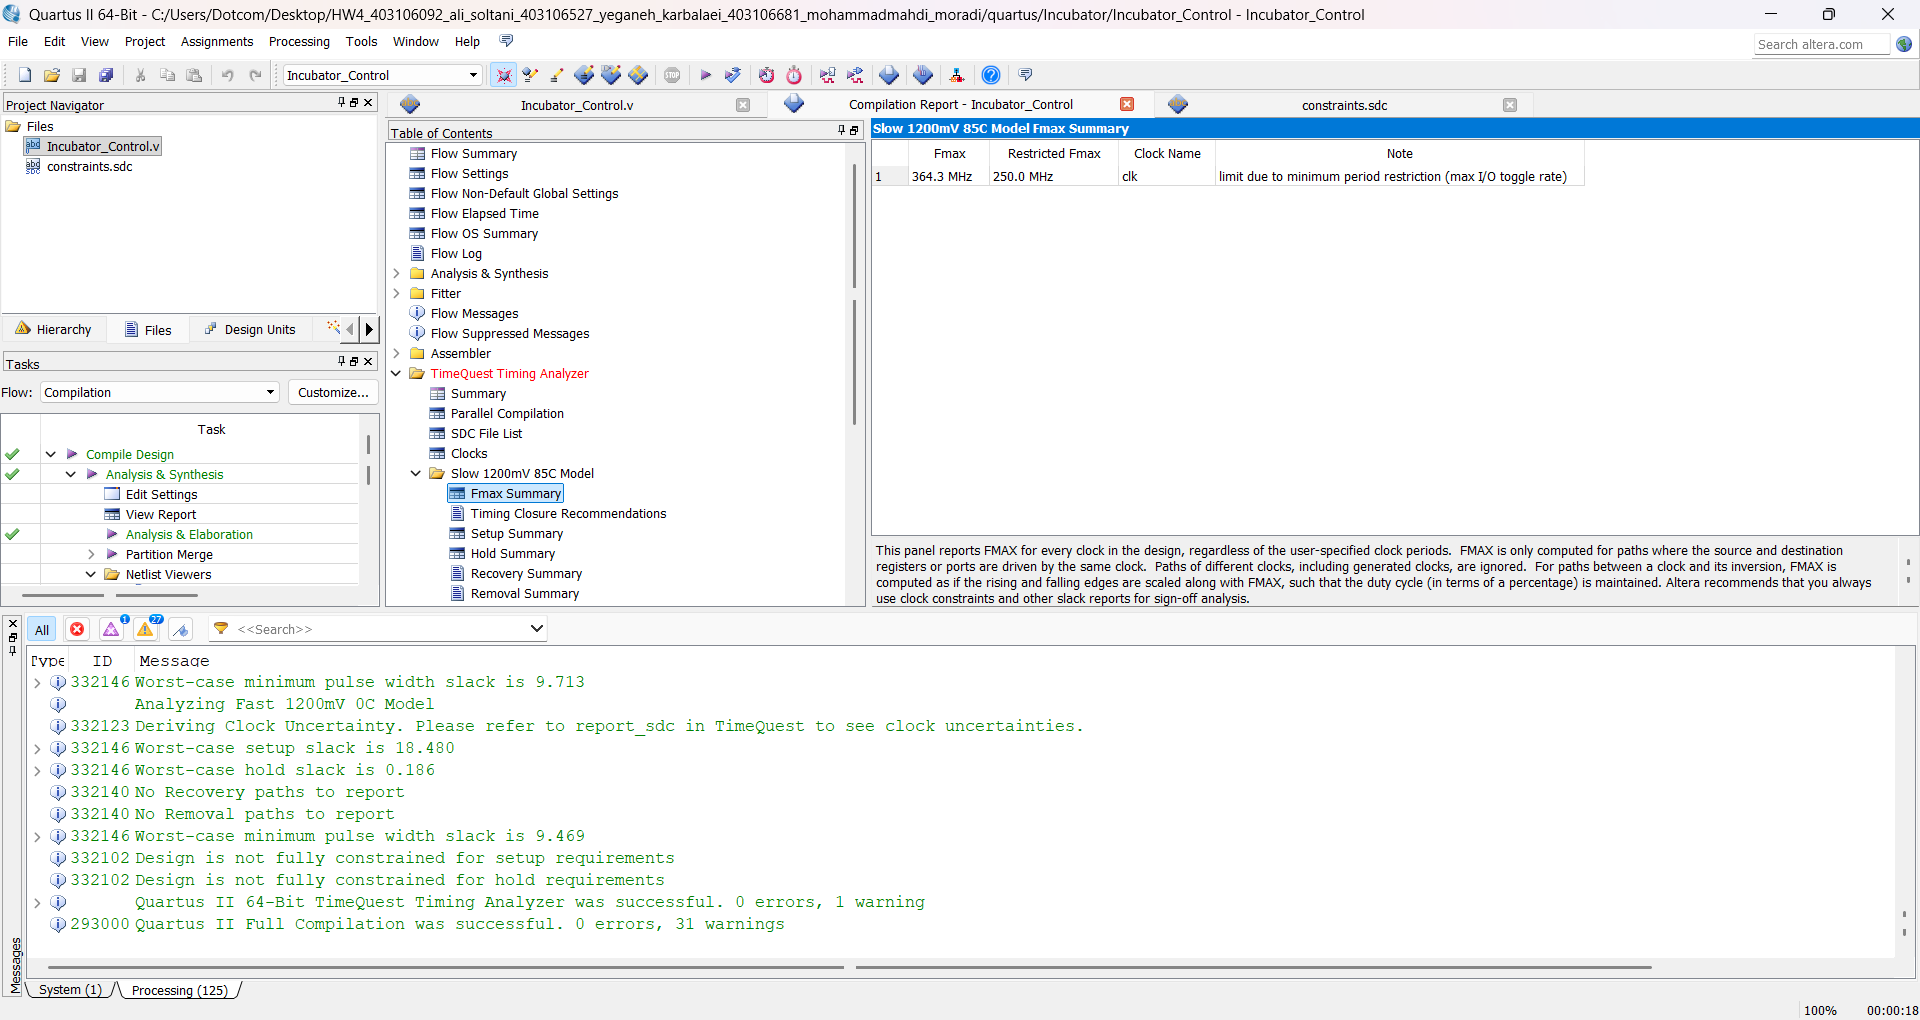
\includegraphics[width=0.9\textwidth]{images/onehot/onehot_fmax_summary.png}
    \caption{بیشینه بسامد کاری در کدگذاری \lr{One-Hot}}
\end{figure}
\begin{figure}[H]
    \centering
    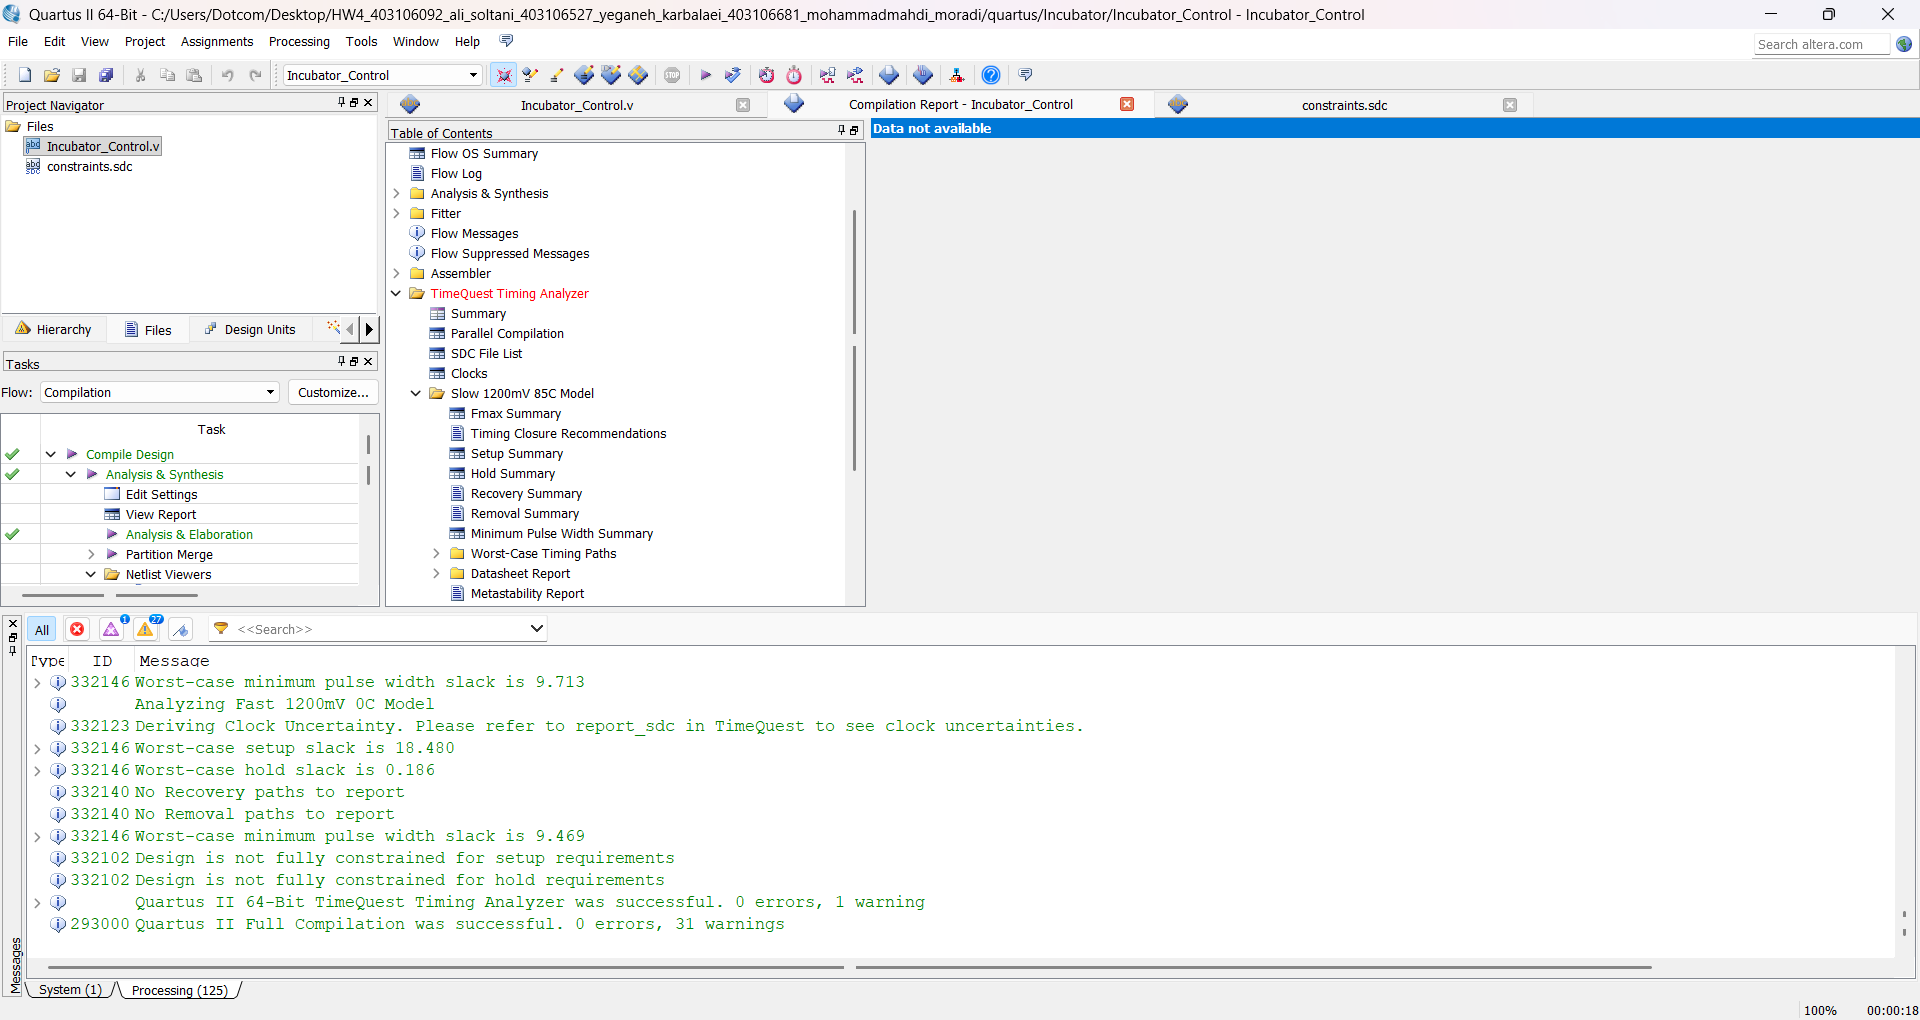
\includegraphics[width=0.9\textwidth]{images/onehot/onehot_setup_summary.png}
    \caption{بررسی \lr{Worst-case slack} در کدگذاری \lr{One-Hot} روی ساعت  \lr{50 MHz}}
\end{figure}

\section{تحلیل نتایج سنتز}
نتایج جدول~\ref{tab:synthesis-results} نشان می‌دهد که کدگذاری \lr{Binary} و \lr{Gray} از نظر تعداد عناصر منطقی و بیشینه بسامد کاری کاملاً یکسان‌اند. علت این است که با تنها چهار حالت، بازنمایی حالت به دو بیت نیاز دارد و منطق گذار حالت بر پایه مقایسه مقدار دما (نه بر پایه مجاورت کدها) نوشته شده است؛ از این رو تعویض ترتیب کدها هیچ تأثیری در ساختار منطق ترکیبی تولیدشده توسط ابزار سنتز ندارد.

در مقابل، کدگذاری \lr{One-Hot} هم عناصر منطقی کمتری مصرف کرده (۲۹ در برابر ۴۳) و هم بیشینه بسامد کاری بالاتری (حدود ۱۴ درصد بهبود) به دست آورده است. علت این پدیده یک قاعده کلی در طراحی رقمی \LTRfootnote{Digital} است: در کدگذاری \lr{One-Hot} هر حالت با یک \lr{flip-flop} مجزا نمایش داده می‌شود، بنابراین برای تشخیص حالت جاری نیازی به رمزگشایی ترکیبی چند بیت با یکدیگر نیست و منطق تولید هر بیت خروجی تنها به تعداد کمی از ورودی‌ها وابسته است. این سادگی، هم تعداد گیت‌های لازم را کاهش می‌دهد و هم با کوتاه‌تر شدن عمق مسیرهای ترکیبی بحرانی، بیشینه بسامد کاری را افزایش می‌دهد. هزینه این روش، افزایش تعداد ثبات هاست (۴ \lr{flip-flop} به‌جای ۲ برای هر ماشین حالت)؛ اما از آنجا که این طرح در مقیاس بسیار کوچکی نسبت به ظرفیت تراشه (۱۴۴۰۰ عنصر منطقی) قرار دارد، این هزینه اضافه، اثر منفی محسوسی در مصرف منابع نداشته و حتی نتیجه کلی هم بهتر شده است.

با توجه به این‌که بسامد کاری موردنیاز این کاربرد بسیار پایین است (خواندن دما تنها هر یک دقیقه یک‌بار)، از منظر عملکردی هر سه روش کدگذاری برای این پروژه کفایت می‌کنند؛ اما در صورت نیاز به بیشینه سرعت ممکن یا کمینه مصرف منابع، \lr{One-Hot} گزینه برتر است.

\section{نتیجه‌گیری}
در این آزمایش، واحد کنترل رقمی یک سامانه انکوباتور شامل دو ماشین حالت (کنترل گرم‌کن/خنک‌کن و کنترل سرعت پنکه) و یک واحد نظارت بر سلامت حسگر با حالت امن طراحی و پیاده‌سازی شد. میزآزمون هوشمند طراحی‌شده با مدل‌سازی رفتار فیزیکی دما، امکان بررسی خودکار عملکرد حلقه بسته کنترل و واکنش سامانه به داده‌های نامعتبر حسگر را فراهم کرد. نتایج شبیه‌سازی نشان داد که منطق طراحی‌شده در تمامی سناریوها (کار عادی، تزریق خطا، بازگشت به کار عادی) به‌درستی عمل می‌کند. مقایسه سه روش کدگذاری حالت نیز نشان داد که در این طرح کوچک، اگرچه \lr{Binary} و \lr{Gray} نتیجه یکسانی دارند، \lr{One-Hot} به‌دلیل ساده‌تر بودن منطق رمزگشایی حالت، هم منابع کمتری مصرف می‌کند و هم بسامد کاری بالاتری ارائه می‌دهد.

\end{document}